\documentclass{beamer}
\mode<presentation>

\usepackage[utf8]{inputenc}
\usepackage[T1]{fontenc}
\usepackage[slovene]{babel}
\usepackage{lmodern}
\usepackage{array} 
\usepackage{tikz}

\usetheme{Berlin}
\usecolortheme{default}
\useinnertheme[shadows]{rounded}
\useoutertheme{infolines}
\beamertemplatenavigationsymbolsempty

\usepackage{times}
\newcommand{\ds}{\displaystyle}
\newcommand{\ts}{\textstyle}
\newcommand{\presledek}{\vspace{3mm}}
\newcommand{\ph}{\phantom{1}} 
\newcommand{\tr}{{\rm tr \,}}

\newtheorem{definicija}{Definicija}
\newtheorem{izrek}{Izrek}
\newtheorem{trditev}{Trditev}


\begin{document}

%%%%%%%%%%%%%%%%%%%%%%%%%%%%%%%%%%%%%%%%%%%%%%%%%%%%%%%%%%%%%%%%%%%%%%%%%%%%%%%%%%%%%%%%%%%%%%%%%%%%%%%%%%%%%%%%%%%%%%%%%%%%%%%%%%%%%%%%%%%%
%%%%%%%%%%%%%%%%%%%%%%%%%%%%%%%%%%%%%%%%%%%%%%%%%%%%%%%%%%%%%%%%%%%%%%%%%%%%%%%%%%%%%%%%%%%%%%%%%%%%%%%%%%%%%%%%%%%%%%%%%%%%%%%%%%%%%%%%%%%%
\title{Statistika v kazenskem pravu}
\subtitle{Dolga predstavitev diplomske naloge}
\author[Neža Kržan]{Neža Kržan}
 
\institute[FMF]{Mentor: izred. prof. dr. Jaka Smrekar \\ Fakulteta za matematiko in fiziko \\ \vspace{10mm} Ljubljana, 5.maj 2023}
\date[5. maj 2023] {}

\subject{Talks}

\begin{frame}
   \titlepage
\end{frame}

%%%%%%%%%%%%%%%%%%%%%%%%%%%%%%%%%%%%%%%%%%%%%%%%%%%%%%%%%%%%%%%%%%%%%%%%%%%%%%%%%%%%%%%%%%%%%%%%%%%%%%%%%%%%%%%%%%%%%%%%%%%%%%%%%%%%%%%%%%%%
%%%%%%%%%%%%%%%%%%%%%%%%%%%%%%%%%%%%%%%%%%%%%%%%%%%%%%%%%%%%%%%%%%%%%%%%%%%%%%%%%%%%%%%%%%%%%%%%%%%%%%%%%%%%%%%%%%%%%%%%%%%%%%%%%%%%%%%%%%%%

%%%%%%%%%%%%%%%%%%%%%%%%%%%%%%%%%%%%%%%%%%%%%%%%%%%%%%%%%%%%%%%%%%%%%%%%%%%%%%%%%%%%%%%%%%%%%%%%%%%%%%%%%%%%%%%%%%%%%%%%%%%%%%%%%%%%%%%%%%%%
%%%%%%%%%%%%%%%%%%%%%%%%%%%%%%%%%%%%%%%%%%%%%%%%%%%%%%%%%%%%%%%%%%%%%%%%%%%%%%%%%%%%%%%%%%%%%%%%%%%%%%%%%%%%%%%%%%%%%%%%%%%%%%%%%%%%%%%%%%%%
\section{Statistika v kazenskem pravu}

\begin{frame}
    \frametitle{Statistika v kazenskem pravu}
    \begin{itemize}
        \item Preverjamo \textbf{teorije} in \textbf{hipoteze}.
        \item Preučujemo razmerja med dvema ali več spremenljivkami.\\ \vspace{2mm}
        \begin{block}{}
            \textbf{Odvisne spremenljivke} - empirični dogodki, ki jih želi raziskovalec pojasniti.\\
            \textbf{Neodvisne spremenljivke} - dejavniki, za katere raziskovalec meni, da bi lahko vplivali na odvisne spremenljivke.
        \end{block}
        \begin{enumerate}
            \item časovno zaporedje;
            \item obstajati mora empirična povezava med odvisno in neodvisno spremenljivko;
            \item razmerje med neodvisno in odvisno spremenljivko nepristransko;
        \end{enumerate}
    \end{itemize}
\end{frame}

%%%%%%%%%%%%%%%%%%%%%%%%%%%%%%%%%%%%%%%%%%%%%%%%%%%%%%%%%%%%%%%%%%%%%%%%%%%%%%%%%%%%%%%%%%%%%%%%%%%%%%%%%%%%%%%%%%%%%%%%%%%%%%%%%%%%%%%%%%%%
\begin{frame}
    \frametitle{Težave}
    \begin{block}{}
        \centering
        Določitev odvisnih in neodvisnih spremenljivk za modeliranje.
    \end{block}
    V proces določanja spremenljivk pogosto posežejo odvetniki, ki se sklicujejo na pravne zakone in načela. To lahko postane sporno, saj lahko takšni 
    posegi ovirajo statistične znanstvenike pri izračunu verjetnostnega vpliva spremenljivk.
\end{frame}

%%%%%%%%%%%%%%%%%%%%%%%%%%%%%%%%%%%%%%%%%%%%%%%%%%%%%%%%%%%%%%%%%%%%%%%%%%%%%%%%%%%%%%%%%%%%%%%%%%%%%%%%%%%%%%%%%%%%%%%%%%%%%%%%%%%%%%%%%%%%
%%%%%%%%%%%%%%%%%%%%%%%%%%%%%%%%%%%%%%%%%%%%%%%%%%%%%%%%%%%%%%%%%%%%%%%%%%%%%%%%%%%%%%%%%%%%%%%%%%%%%%%%%%%%%%%%%%%%%%%%%%%%%%%%%%%%%%%%%%%%
\section{Uporaba statistike pri pravnem postopku}

\begin{frame}
    \frametitle{Uporaba statistike pri pravnem postopku}
    Pred pričanjem na sodišču moramo vedeti
    \begin{enumerate}
        \item na kaj točno se podatki nanašajo,
        \item kako so bili zbrani,
        \item kakšen del podatkov manjka ali je neuporaben.
    \end{enumerate}
    $\Rightarrow$ \textbf{Določimo ustrezen postopek analize podatkov.}\\ \vspace{3mm}
    Potrebujemo
    \begin{enumerate}
        \item osnovne informacije odvetnika in drugih strokovnjakov,
        \item določitev ustrezne populacije,
        \item določitev parametrov, ki nas zanimajo,
        \item določitev statističnega postopka.
    \end{enumerate}
    $\Rightarrow$ \textbf{Oblikujemo ustrezne primerjalne skupine.}
\end{frame}

%%%%%%%%%%%%%%%%%%%%%%%%%%%%%%%%%%%%%%%%%%%%%%%%%%%%%%%%%%%%%%%%%%%%%%%%%%%%%%%%%%%%%%%%%%%%%%%%%%%%%%%%%%%%%%%%%%%%%%%%%%%%%%%%%%%%%%%%%%%%%%
%%%%%%%%%%%%%%%%%%%%%%%%%%%%%%%%%%%%%%%%%%%%%%%%%%%%%%%%%%%%%%%%%%%%%%%%%%%%%%%%%%%%%%%%%%%%%%%%%%%%%%%%%%%%%%%%%%%%%%%%%%%%%%%%%%%%%%%%%%%%%%
\section{Raziskovalni proces}
\begin{frame}
    \frametitle{Raziskovalni proces}
    Raziskovalni proces v kazenskem pravosodju je običajno namenjen preučevanju problemov kriminala. Proces se izvaja po naslednjih točkah.\\ \vspace{2mm}
    \begin{enumerate}
        \item \textbf{Identifikacija problema.\\} 
        \item \textbf{Zasnova raziskave.\\} 
        \item \textbf{Analiza podatkov.\\}
    \end{enumerate}
\end{frame}

%%%%%%%%%%%%%%%%%%%%%%%%%%%%%%%%%%%%%%%%%%%%%%%%%%%%%%%%%%%%%%%%%%%%%%%%%%%%%%%%%%%%%%%%%%%%%%%%%%%%%%%%%%%%%%%%%%%%%%%%%%%%%%%%%%%%%%%%%%%%%%
%%%%%%%%%%%%%%%%%%%%%%%%%%%%%%%%%%%%%%%%%%%%%%%%%%%%%%%%%%%%%%%%%%%%%%%%%%%%%%%%%%%%%%%%%%%%%%%%%%%%%%%%%%%%%%%%%%%%%%%%%%%%%%%%%%%%%%%%%%%%%%
\section{Vrednotenje dokazov}
\begin{frame}
    \frametitle{Vrednotenje dokazov}
    \begin{block}{Dokazni standard}
        je pravno vprašanje. Gre za abstraktno normo, ki je (podobno kot obstoj določenih predpostavk za 
        določeno kaznivo dejanje) opredeljena s pravnim pravilom.
    \end{block}\vspace{3mm}
    \textbf{METODA DOKAZNE VREDNOSTI}\\
    \textbf{MODEL VERJETNOSTI HIPOTEZE}\\ \vspace{3mm}
    V kazenskem pravu lahko zelo hitro pride do posebnih, edinstvenih predpostavk oziroma hipotez, ki pa predstavljajo težave pri vrednotenju oziroma merjenju v statističnih modelih. 
\end{frame}


%%%%%%%%%%%%%%%%%%%%%%%%%%%%%%%%%%%%%%%%%%%%%%%%%%%%%%%%%%%%%%%%%%%%%%%%%%%%%%%%%%%%%%%%%%%%%%%%%%%%%%%%%%%%%%%%%%%%%%%%%%%%%%%%%%%%%%%%%%%%
%%%%%%%%%%%%%%%%%%%%%%%%%%%%%%%%%%%%%%%%%%%%%%%%%%%%%%%%%%%%%%%%%%%%%%%%%%%%%%%%%%%%%%%%%%%%%%%%%%%%%%%%%%%%%%%%%%%%%%%%%%%%%%%%%%%%%%%%%%%%
\section{Koncept verjetnosti}

\begin{frame}
    \frametitle{Koncept verjetnosti}
    Opravlja se primerjava verjetnosti dokazov na podlagi dveh konkurenčnih predlogov:\\
    $H_p \dots$ trditev, ki jo predlaga tožilstvo;\\
    $H_d \dots$ trditev, ki jo predlaga obramba.\\ \vspace{5mm}
    Koncept verjetnosti je
    \begin{itemize}
        \item ključen pri ocenjevanju dokazov;
        \item omogoča objektivno oceno vpliva dokaza na verjetnost določene domneve o interesni osebi ali obdolžencu.
    \end{itemize}
\end{frame}

%%%%%%%%%%%%%%%%%%%%%%%%%%%%%%%%%%%%%%%%%%%%%%%%%%%%%%%%%%%%%%%%%%%%%%%%%%%%%%%%%%%%%%%%%%%%%%%%%%%%%%%%%%%%%%%%%%%%%%%%%%%%%%%%%%%%%%%%%%%%
\begin{frame}
    \frametitle{Presoja dokazov}
    \begin{itemize}
        \item Za presojo se uporabljajo različne metode in tehnike, ki temeljijo na statistični verjetnosti,
        \item metode omogočajo oceno, kako verjetno je, da so dokazi resnični in zanesljivi. 
    \end{itemize}
    \begin{beamerboxesrounded}[]{KONTEKST DOKAZA}
        \begin{itemize}
            \item Upoštevamo druge dokaze in okoliščine primera.
            \item Izvedemo bolj objektivno presojo dokazov.
            \item Vpliv na določeno domnevo oziroma hipotezo o interesni osebi ali obdolžencu.
            \item Upoštevamo verjetnost napake - verjetnost, da so dokazi napačni ali zavajajoči.
        \end{itemize} 
    \end{beamerboxesrounded}
\end{frame}

%%%%%%%%%%%%%%%%%%%%%%%%%%%%%%%%%%%%%%%%%%%%%%%%%%%%%%%%%%%%%%%%%%%%%%%%%%%%%%%%%%%%%%%%%%%%%%%%%%%%%%%%%%%%%%%%%%%%%%%%%%%%%%%%%%%%%%%%%%%%
\begin{frame}
    \frametitle{Koncept verjetnosti}
    \begin{beamerboxesrounded}[]{Verjetnost proti nedolžnosti ali verjetnost za krivdo}
        \[
            \frac{P(H_p)}{P(H_d)}
        \]    
    \end{beamerboxesrounded} \vspace{3mm}
    \begin{beamerboxesrounded}[]{Verjetnost v prid krivdi ob upoštevanju informacij $E$}
        \[
            \frac{P(H_p \lvert E)}{P(H_d \lvert E)} 
        \]    
    \end{beamerboxesrounded} \vspace{5mm}
    Če imamo na voljo dokaz $E$, nas zanima pogojna verjetnost
    \[
        P(kriv \lvert E), \vspace{2mm}
    \]
    pri čemer nam je lahko v pomoč Bayesovo pravilo.
\end{frame}

%%%%%%%%%%%%%%%%%%%%%%%%%%%%%%%%%%%%%%%%%%%%%%%%%%%%%%%%%%%%%%%%%%%%%%%%%%%%%%%%%%%%%%%%%%%%%%%%%%%%%%%%%%%%%%%%%%%%%%%%%%%%%%%%%%%%%%%%%%%%
%%%%%%%%%%%%%%%%%%%%%%%%%%%%%%%%%%%%%%%%%%%%%%%%%%%%%%%%%%%%%%%%%%%%%%%%%%%%%%%%%%%%%%%%%%%%%%%%%%%%%%%%%%%%%%%%%%%%%%%%%%%%%%%%%%%%%%%%%%%%
\section{Bayesova statistika}

%%%%%%%%%%%%%%%%%%%%%%%%%%%%%%%%%%%%%%%%%%%%%%%%%%%%%%%%%%%%%%%%%%%%%%%%%%%%%%%%%%%%%%%%%%%%%%%%%%%%%%%%%%%%%%%%%%%%%%%%%%%%%%%%%%%%%%%%%%%%
\begin{frame}
    \frametitle{Bayesova teorija v kazenskem pravu}
    Bayesovo sklepanje razlaga verjetnost kot merilo verjetnosti ali zaupanja, ki ga lahko ima posameznik glede nastanka določenega dogodka.
    \begin{itemize}
      \item O dogodku lahko že imamo predhodno prepričanje oziroma apriorno prepričanje.
      \item Ta se lahko spremeni, ko se pojavijo novi dokazi.
    \end{itemize} \vspace{3mm}
    Bayesova statistika nam daje matematične modele za vključevanje naših apriornih prepričanj in dokazov za ustvarjanje novih prepričanj.
\end{frame}

\begin{frame}
    \frametitle{Bayesova teorija v kazenskem pravu}
    Ocena, kako informacije vplivajo na tožilčevo domnevo o obdolžencu oziroma storilcu kaznivega dejanja. \\ \vspace{3mm}
    Postopek posodabljanja verjetnosti tožilčeve hipoteze na podlagi predhodnih oziroma apriornih verjetnosti. \\ \vspace{3mm}
    \begin{block}{}
        \centering
        verjetnost hipoteze pred upoštevanjem določenega dokaza (dokazov) \\ \vspace{2mm}
        $\Rightarrow$ \\ \vspace{3mm}
        verjetnost hipoteze po upoštevanju določenega dokaza (dokazov)
    \end{block}
\end{frame}

%%%%%%%%%%%%%%%%%%%%%%%%%%%%%%%%%%%%%%%%%%%%%%%%%%%%%%%%%%%%%%%%%%%%%%%%%%%%%%%%%%%%%%%%%%%%%%%%%%%%%%%%%%%%%%%%%%%%%%%%%%%%%%%%%%%%%%%%%%%%
\begin{frame}
    \frametitle{Predhodna verjetnost in določitev posteriorne verjetnosti}
    \begin{block}{Predhodna verjetnost}
        začetna verjetnost hipoteze oziroma tožilčeve domneve o obdolžencu oziroma storilcu kaznivega dejanja.
    \end{block} \vspace{3mm}
    \begin{block}{Predhodna verjetnost}
        verjetnost začetne hipoteze oziroma tožilčeve domneve o obdolžencu, preden so bili predloženi dokazi.
    \end{block}
\end{frame}

%%%%%%%%%%%%%%%%%%%%%%%%%%%%%%%%%%%%%%%%%%%%%%%%%%%%%%%%%%%%%%%%%%%%%%%%%%%%%%%%%%%%%%%%%%%%%%%%%%%%%%%%%%%%%%%%%%%%%%%%%%%%%%%%%%%%%%%%%%%%
\begin{frame}
    \frametitle{Težave z določitvijo predhodne verjetnosti}
    Različne metode za določitev in izračun predhodnih verjetnosti lahko dajejo različne rezultate. \\ \vspace{3mm}
    \begin{block}{Ali naj analitiki poskušajo določiti predhodne verjetnosti in če ja, kako naj jih določijo?}
        \begin{itemize}
            \item \textbf{Nevtralno stanje} - analitiki predpostavi enake predhodne verjetnosti za vse hipoteze v primeru;
            \item Analitik naj uporabi svoje strokovno znanje za izračun apriorne verjetnosti na podlagi razpoložljivih podatkov in brez nepotrebnega vplivanja odvetnikov ali drugih udeležencev postopka;
        \end{itemize}
    \end{block}
\end{frame}

%%%%%%%%%%%%%%%%%%%%%%%%%%%%%%%%%%%%%%%%%%%%%%%%%%%%%%%%%%%%%%%%%%%%%%%%%%%%%%%%%%%%%%%%%%%%%%%%%%%%%%%%%%%%%%%%%%%%%%%%%%%%%%%%%%%%%%%%%%%%
%%%%%%%%%%%%%%%%%%%%%%%%%%%%%%%%%%%%%%%%%%%%%%%%%%%%%%%%%%%%%%%%%%%%%%%%%%%%%%%%%%%%%%%%%%%%%%%%%%%%%%%%%%%%%%%%%%%%%%%%%%%%%%%%%%%%%%%%%%%%
\section{Drugi pristopi}

\begin{frame}
    \frametitle{Frekvence}
    \begin{itemize}
        \item frekvence se običajno nanašajo na pojavljanje dokazov za posamezen primer;
        \item sklepanje o krivdi je lahko podprto s verjetnostnim sklepanjem z uporabo absolutnih ali relativnih frekvenc;
    \end{itemize}
    \begin{block}{Relativne frekvence}
        \begin{itemize}
            \item navajajo (predpostavljajo) obstoj referenčnega vzorca, na podlagi katerega se lahko oceni pogostost zadevnega dogodka;
            \item lahko podpre vmesno sklepanje o moči dokazov;
            \item rutinsko vključene v znanstvene dokaze.
        \end{itemize}  
    \end{block}
\end{frame}

%%%%%%%%%%%%%%%%%%%%%%%%%%%%%%%%%%%%%%%%%%%%%%%%%%%%%%%%%%%%%%%%%%%%%%%%%%%%%%%%%%%%%%%%%%%%%%%%%%%%%%%%%%%%%%%%%%%%%%%%%%%%%%%%%%%%%%%%%%%%
\begin{frame}
    \frametitle{Frekvence}
    \begin{itemize}
        \item \textbf{teoretična pomanjkljivost} - zahtevajo statistične dokaze, ki sodišču niso na voljo;
        \item frekvenčni modeli temeljijo na predpostavki, a visoka vrednost verjetnosti, ki opisuje razmerje med obstoječimi dokazi in primerom, pomeni, da je vrednost tega dokaza visoka;
        \item uporaba frekvenčnih modelov je lahko zelo omejena;
    \end{itemize} \vspace{3mm}
\end{frame}

%%%%%%%%%%%%%%%%%%%%%%%%%%%%%%%%%%%%%%%%%%%%%%%%%%%%%%%%%%%%%%%%%%%%%%%%%%%%%%%%%%%%%%%%%%%%%%%%%%%%%%%%%%%%%%%%%%%%%%%%%%%%%%%%%%%%%%%%%%%%
\begin{frame}
    \frametitle{Metoda verjetnosti naključnega ujemanja}
    \begin{block}{}
        Izraža možnost, da bi imel naključni posameznik, ki ni povezan z obdolžencem, ustrezni DNK profil. Ta verjetnost je enaka pogostosti profila DNK. 
    \end{block}\vspace{2mm}
    Pogosto se to verjetnost interpretira kot:
    \begin{enumerate}
        \item če je verjetnost naključnega ujemanja na primer 1 proti 100 milijonom, potem je verjetnost, da ima profil DNK drug posameznik in ne
        obdolženec 1 proti 100 milijonom;
        \item ker je to zelo majhna verjetnost, mora biti tudi verjetnost, da je sled DNK pustil nekdo drug na kraju zločina in ne obdolženec, zelo majhna;
        \item zato mora biti verjetnost, da je vir sledi DNK s kraja zločina obtoženec zelo velika, ampak znaša 1 proti 100 milijonov.
    \end{enumerate} \vspace{2mm}
    \begin{block}{}
        \centering
        $\Rightarrow$ \textbf{TOŽILČEVA ZMOTA}
    \end{block} 
\end{frame}

%%%%%%%%%%%%%%%%%%%%%%%%%%%%%%%%%%%%%%%%%%%%%%%%%%%%%%%%%%%%%%%%%%%%%%%%%%%%%%%%%%%%%%%%%%%%%%%%%%%%%%%%%%%%%%%%%%%%%%%%%%%%%%%%%%%%%%%%%%%%
%%%%%%%%%%%%%%%%%%%%%%%%%%%%%%%%%%%%%%%%%%%%%%%%%%%%%%%%%%%%%%%%%%%%%%%%%%%%%%%%%%%%%%%%%%%%%%%%%%%%%%%%%%%%%%%%%%%%%%%%%%%%%%%%%%%%%%%%%%%%
\section{Razmerje verjetnosti}

%%%%%%%%%%%%%%%%%%%%%%%%%%%%%%%%%%%%%%%%%%%%%%%%%%%%%%%%%%%%%%%%%%%%%%%%%%%%%%%%%%%%%%%%%%%%%%%%%%%%%%%%%%%%%%%%%%%%%%%%%%%%%%%%%%%%%%%%%%%%
\begin{frame}
    \frametitle{Razmerje verjetnosti v kazenskem pravu}
    $H_p \dots$ interesna oseba oz. obtoženec je resnično kriv - nadomestimo $H$;\\
    $H_d \dots$ interesna oseba je resnično nedolžen - nadomestimo $\bar{H}$;\\
    $Ev \dots$ obravnavani dokaz - nadomestimo dogodek $E$;\\
    \begin{block}{Bayesovov izreka omogoča, da se predhodne verjetnosti v korist krivde posodobijo v posteriorne verjetnosti}
        \[
            \frac{P(H_p \lvert Ev)}{P(H_d \lvert Ev)} = \frac{P(Ev \lvert H_p)}{P(Ev \lvert H_d)} \times \frac{P(H_p)}{P(H_d)}. \vspace{2mm}
        \]
    \end{block}\vspace{2mm}
    \begin{block}{Ob upoštevanju informacij $I$}
        \[
            \frac{P(H_p \lvert Ev, I)}{P(H_d \lvert Ev, I)} = \frac{P(Ev \lvert H_p, I)}{P(Ev \lvert H_d, I)} \times \frac{P(H_p \lvert I)}{P(H_d \lvert I)}. \vspace{2mm}
        \]
    \end{block}
\end{frame}

\begin{frame}
    \frametitle{Razmerje verjetnosti v kazenskem pravu}
    \begin{definicija}
        Naj bosta  $H_p$ in $H_d$ dve konkurenčni hipotezi ter $I$ informacije o ozadju. Vrednost $V$ dokaza $Ev$ je podana z
        \[
            V = \frac{P(Ev \lvert H_p, I)}{P(Ev \lvert H_d, I)},
        \]
        razmerje verjetnosti, ki pretvori predhodne verjetnosti
        \[
            \frac{P(H_p \lvert I)}{P(H_d \lvert I)} 
        \]
        v posteriorne verjetnosti
        \[
            \frac{P(H_p \lvert Ev, I)}{P(H_d \lvert Ev, I)}.
        \]
     \end{definicija}     
\end{frame}

%%%%%%%%%%%%%%%%%%%%%%%%%%%%%%%%%%%%%%%%%%%%%%%%%%%%%%%%%%%%%%%%%%%%%%%%%%%%%%%%%%%%%%%%%%%%%%%%%%%%%%%%%%%%%%%%%%%%%%%%%%%%%%%%%%%%%%%%%%%%
\begin{frame}
    \frametitle{Utemeljitev uporabe razmerja verjetnosti}
    \begin{enumerate}
        \item katera hipoteza je bolje podprta z dokazi;
        \item v primerih, ko je treba združiti več hipotez in/ali več dokazov;
        \item za količinsko ovrednotenje skupnega učinka več dokazov, ki vključujejo različne povezane hipoteze;
    \end{enumerate} \vspace{3mm}
    \begin{block}{Negotovosti}
        \begin{itemize}
            \item kakovost podatkov, pridobljenih z analizami;
            \item izbira kontrolnega vzorca;
            \item osebno poznavanje okoliščin iz določenega primera;
            \item pridobivanje predhodnih verjetnosti, pogojenih z razpoložljivim znanjem;
            \item numerični postopki za razreševanje računskih težav;
        \end{itemize}
    \end{block} \vspace{2mm}
    \centering
    $\Rightarrow$ \textbf{poročilo vključuje merilo njegove natančnosti}
\end{frame}

%%%%%%%%%%%%%%%%%%%%%%%%%%%%%%%%%%%%%%%%%%%%%%%%%%%%%%%%%%%%%%%%%%%%%%%%%%%%%%%%%%%%%%%%%%%%%%%%%%%%%%%%%%%%%%%%%%%%%%%%%%%%%%%%%%%%%%%%%%%%
%%%%%%%%%%%%%%%%%%%%%%%%%%%%%%%%%%%%%%%%%%%%%%%%%%%%%%%%%%%%%%%%%%%%%%%%%%%%%%%%%%%%%%%%%%%%%%%%%%%%%%%%%%%%%%%%%%%%%%%%%%%%%%%%%%%%%%%%%%%%
\section{Zmote v kazenskem pravu}

\begin{frame}
    \frametitle{Zmote v kazenskem pravu}
    Če upoštevamo vzročno verigo dokazov, predstavljeno na sliki, lahko razvrstitev zmot posplošimo na večino vrst dokazov. 
    \begin{figure}[!ht]\label{fig:slika_3}
        \centering
        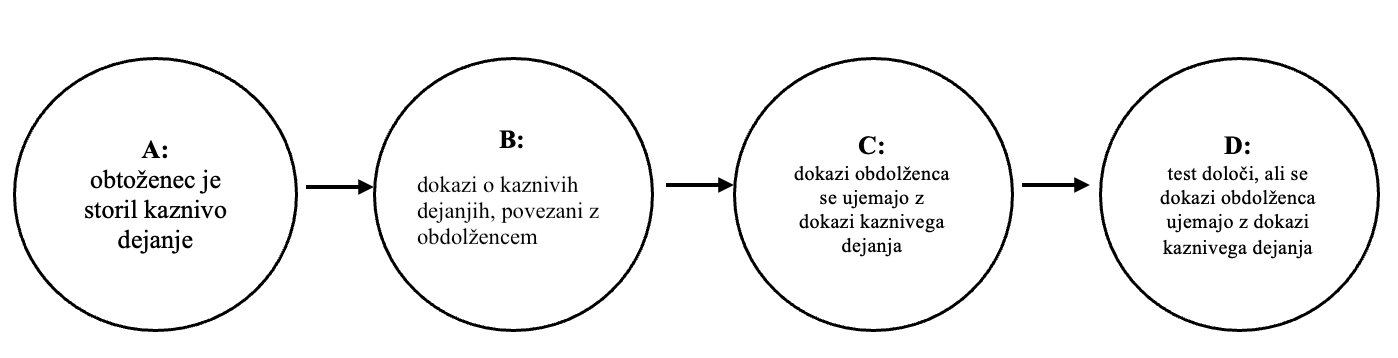
\includegraphics[scale=0.50]{slika_3.png}
        \caption{Vzorčna veriga dokazov}
    \end{figure}
\end{frame}

\begin{frame}
    \frametitle{Zmote v kazenskem pravu}
    \begin{block}{Tožilčeva zmota}
        enačimo $P(C \lvert \neg B)$ s $P(\neg A \lvert C)$.
    \end{block}
    \begin{figure}[!ht]\label{fig:slika_3}
        \centering
        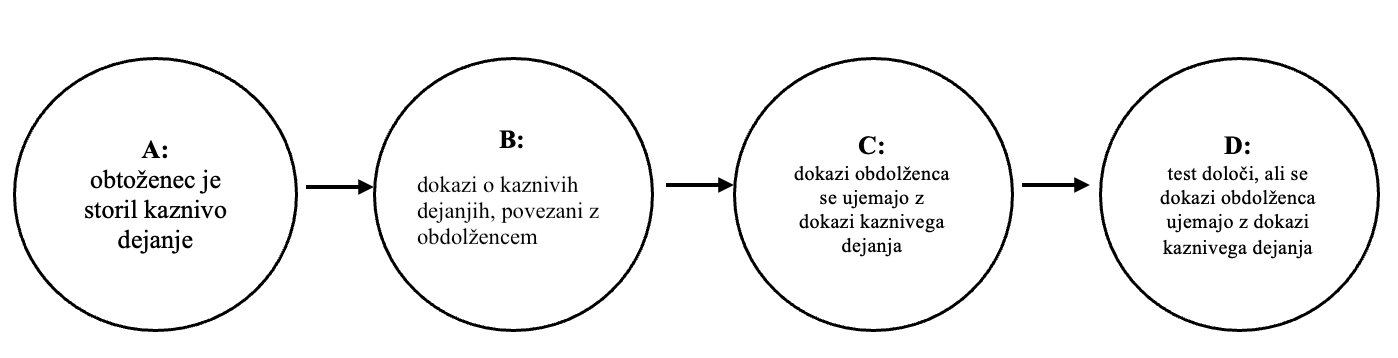
\includegraphics[scale=0.50]{slika_3.png}
        \caption{Vzorčna veriga dokazov}
    \end{figure}
\end{frame}

\begin{frame}
    \frametitle{Zmote v kazenskem pravu}
    \begin{block}{Napaka verjetnosti}
        $P(C \lvert \neg B)$ enačimo z verjetnostjo (imenujmo jo $q$), da ima vsaj en nedolžen član populacije ustreza dokazom.
    \end{block}
    \begin{figure}[!ht]\label{fig:slika_3}
        \centering
        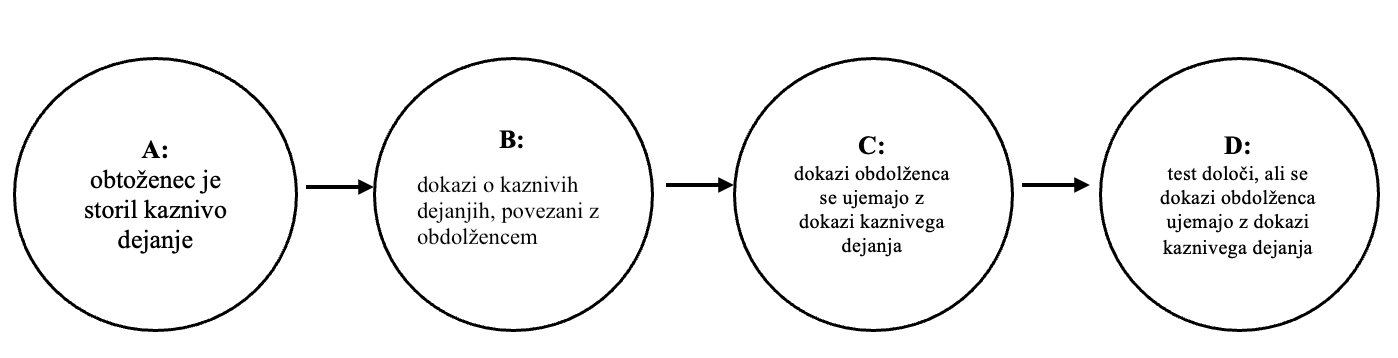
\includegraphics[scale=0.50]{slika_3.png}
        \caption{Vzorčna veriga dokazov}
    \end{figure}
\end{frame}

\begin{frame}
    \frametitle{Zmote v kazenskem pravu}
    \begin{block}{Zanemarjanje predhodnih verjetnosti}
        neupoštevanje predhodnih vrednosti, kot sta $P(A)$ in $P(B)$.
    \end{block}
    \begin{figure}[!ht]\label{fig:slika_3}
        \centering
        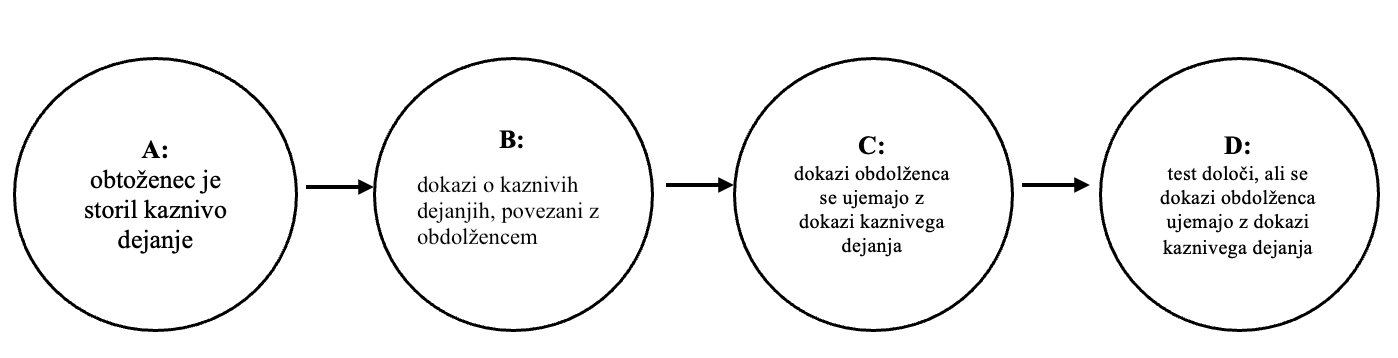
\includegraphics[scale=0.50]{slika_3.png}
        \caption{Vzorčna veriga dokazov}
    \end{figure}
\end{frame}

\begin{frame}
    \frametitle{Zmote v kazenskem pravu}
    \begin{block}{Napaka pri številčnem preračunavanju}
        gre za zamenjavo vrednosti $P(C \lvert \neg B)$ s pričakovanim številom drugih oseb, ki bi jih bilo treba testirati, preden bi našli ujemanje.
    \end{block}
    \begin{figure}[!ht]\label{fig:slika_3}
        \centering
        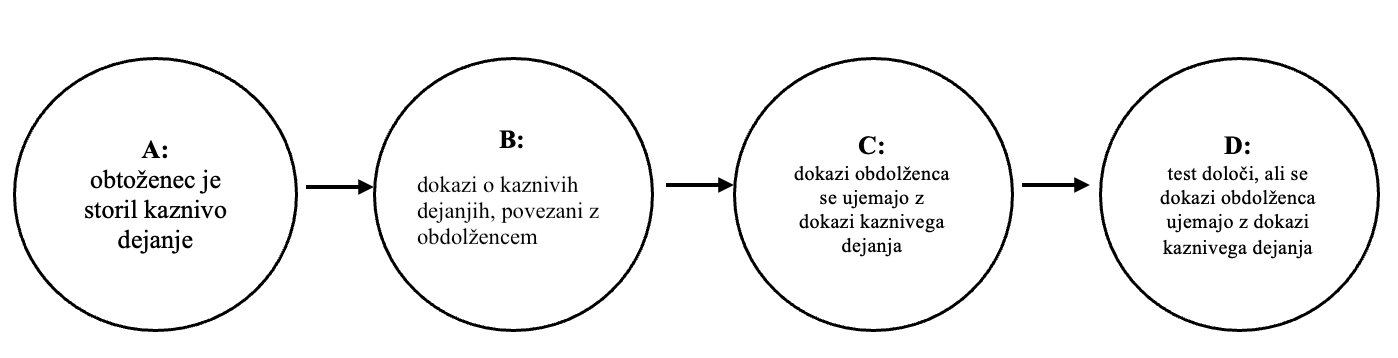
\includegraphics[scale=0.50]{slika_3.png}
        \caption{Vzorčna veriga dokazov}
    \end{figure}
\end{frame}

\begin{frame}
    \frametitle{Zmote v kazenskem pravu}
    \begin{block}{Pričakovane vrednosti, ki pomenijo edinstvenost}
        če je velikost populacije približno enaka $1/P(\neg B \lvert C)$, potem mora biti
        obdolženec edini primerek.
    \end{block}
    \begin{figure}[!ht]\label{fig:slika_3}
        \centering
        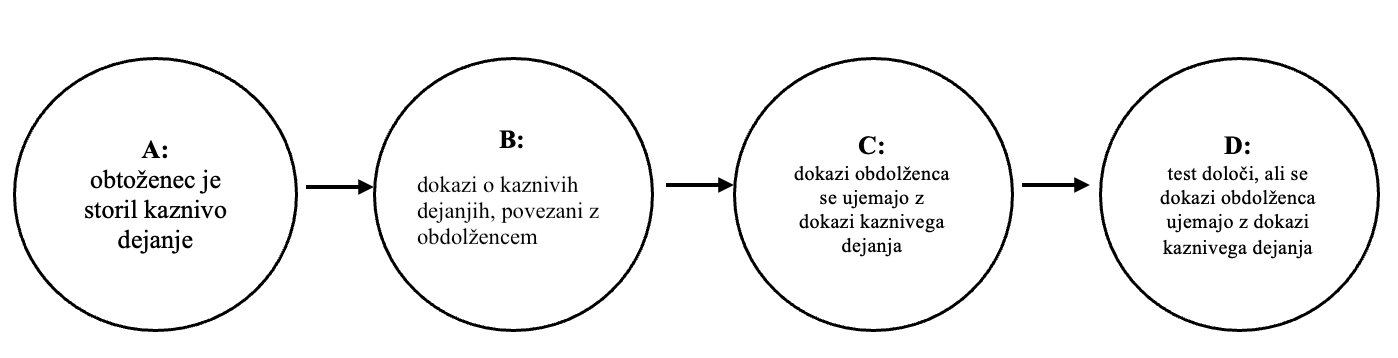
\includegraphics[scale=0.50]{slika_3.png}
        \caption{Vzorčna veriga dokazov}
    \end{figure}
\end{frame}

\begin{frame}
    \frametitle{Zmote v kazenskem pravu}
    \begin{block}{Zmota obrambnega odvetnika}
        dokaz $C$ štejemo za nepomembnega, ker visoka predhodna verjetnost $P(\neg A)$ še vedno povzroči visoko verjetnost $P(\neg B \lvert C)$.    
    \end{block}
    \begin{figure}[!ht]\label{fig:slika_3}
        \centering
        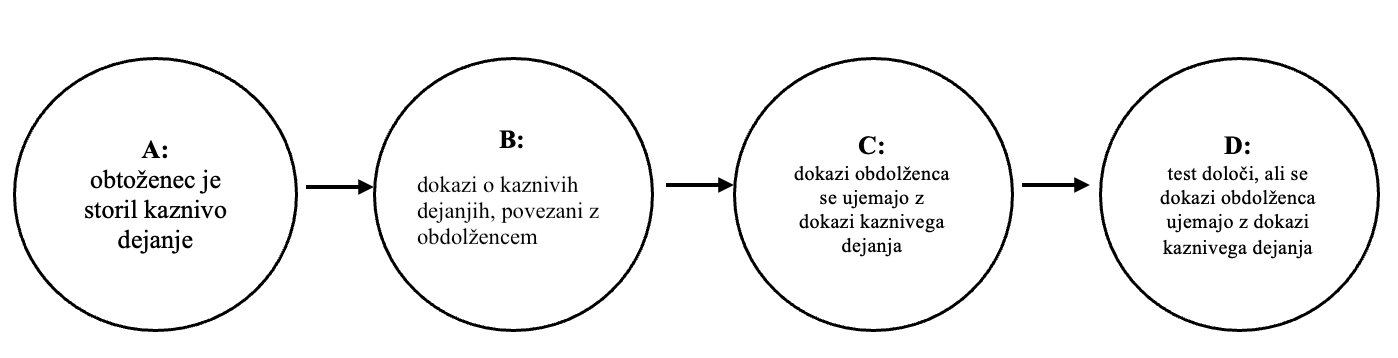
\includegraphics[scale=0.50]{slika_3.png}
        \caption{Vzorčna veriga dokazov}
    \end{figure}
\end{frame}

\begin{frame}
    \frametitle{Zmote v kazenskem pravu}
    \begin{block}{Napaka baze podatkov obrambnega odvetnika}
        verjetnost $P(\neg B \lvert C)$ temelji na drugačni populaciji, kot jo določa $P(B)$ ali $P(A)$.    
    \end{block}
    \begin{figure}[!ht]\label{fig:slika_3}
        \centering
        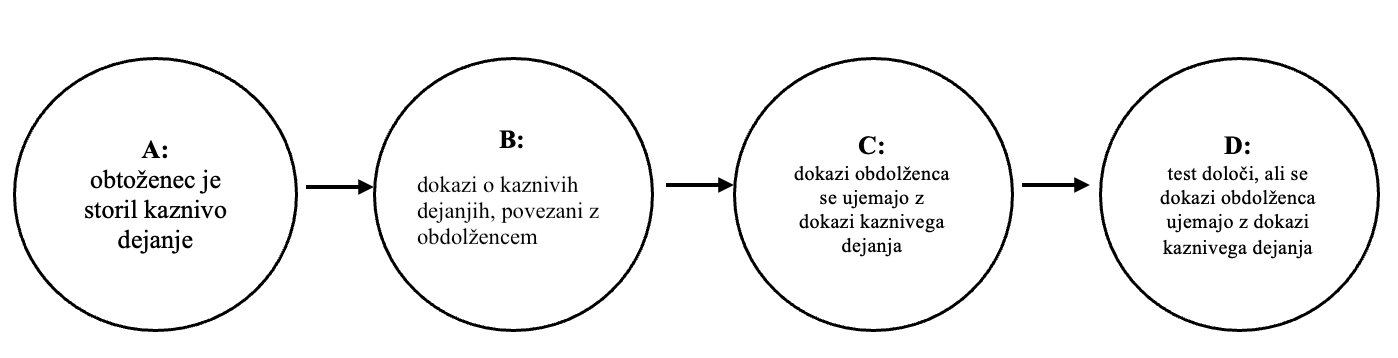
\includegraphics[scale=0.50]{slika_3.png}
        \caption{Vzorčna veriga dokazov}
    \end{figure}
\end{frame}

\begin{frame}
    \frametitle{Zmote v kazenskem pravu}
    \begin{block}{Zasliševalčeva zmota}
        v tem primeru je dokaz neposredno priznanje krivde. Če to ni potrjeno, to pomeni, da uporabljamo $P(D \lvert A)$ za
        informiranje $P(A \lvert D)$. Napaka je, da ne upoštevamo $P(D \lvert \neg A)$. Če je $P(D \lvert A) \leq P(D \lvert \neg A)$, potem dokaz
        nima vrednosti.    
    \end{block}
    \begin{figure}[!ht]\label{fig:slika_3}
        \centering
        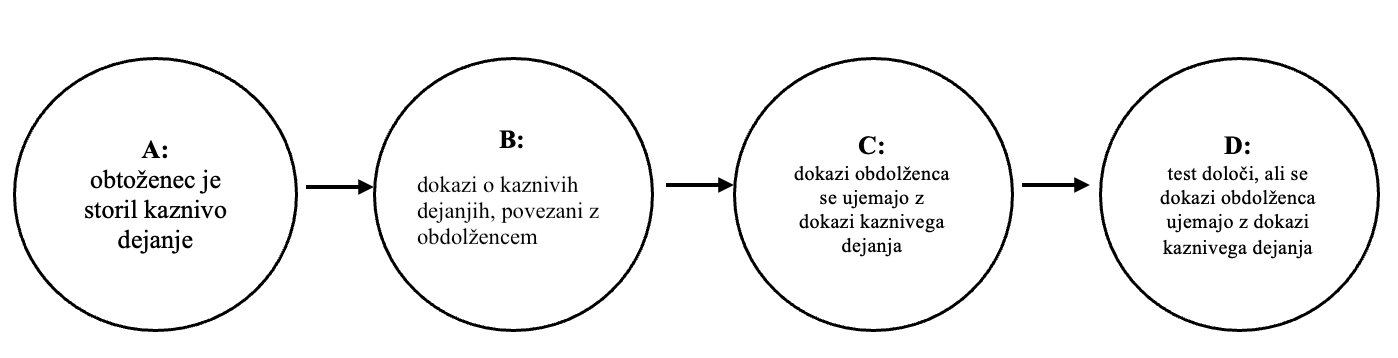
\includegraphics[scale=0.40]{slika_3.png}
        \caption{Vzorčna veriga dokazov}
    \end{figure}
\end{frame}

%%%%%%%%%%%%%%%%%%%%%%%%%%%%%%%%%%%%%%%%%%%%%%%%%%%%%%%%%%%%%%%%%%%%%%%%%%%%%%%%%%%%%%%%%%%%%%%%%%%%%%%%%%%%%%%%%%%%%%%%%%%%%%%%%%%%%%%%%%%%
%%%%%%%%%%%%%%%%%%%%%%%%%%%%%%%%%%%%%%%%%%%%%%%%%%%%%%%%%%%%%%%%%%%%%%%%%%%%%%%%%%%%%%%%%%%%%%%%%%%%%%%%%%%%%%%%%%%%%%%%%%%%%%%%%%%%%%%%%%%%
\section{Načini za izogib zmotam}

%%%%%%%%%%%%%%%%%%%%%%%%%%%%%%%%%%%%%%%%%%%%%%%%%%%%%%%%%%%%%%%%%%%%%%%%%%%%%%%%%%%%%%%%%%%%%%%%%%%%%%%%%%%%%%%%%%%%%%%%%%%%%%%%%%%%%%%%%%%%
\begin{frame}
    \frametitle{Izogibanje zmotam z uporabo Bayesovih omrežij}
    \begin{block}{}
        Bayesova omrežja pomagajo določiti ustrezne verjetnostne formule, ne da bi prikazali njihovo polno algebrsko obliko, in omogočajo skoraj popolno avtomatizacijo potrebnih verjetnostnih izračunov.
    \end{block} \vspace{3mm}
    \begin{enumerate}
        \item med konkurenčnimi hipotezami izberemo najverjetnejšo;
        \item izbira mora biti podprta z znanstveno utemeljeno argumentacijo;
        \item primerna so za analizo dogodka;
        \item primerno za napovedovanje verjetnosti, da je k dogodku prispeval katerikoli od več možnih znanih vzrokov;
    \end{enumerate}
    \begin{block}{}
        Prednosti Bayesovih mrež se najbolj izrazito pokažejo na zapletenih področjih z več spremenljivkami.
    \end{block}
\end{frame}

\begin{frame}
    \frametitle{Izogibanje zmotam z uporabo Bayesovih omrežij}
    \begin{itemize}
        \item bistveno izboljšajo vrednotenje verjetnostnih razmerij, ki se uporabljajo za ocenjevanje znanstvenih dokazov;
        \item omogočajo kompleksnejše verjetnostne analize;
        \item če se za izdelavo ne uporablja dosleden okvir, lahko Bayesovo omrežje kaže različne rezultate;
    \end{itemize} \vspace{3mm}
    \begin{block}{}
        Prikaz Bayesovega omrežja se mora ujemati z intuitivnim pripisovanjem vzročno-posledičnih povezav med končno hipotezo, podhipotezo in dokazi primera.
    \end{block}
\end{frame}

%%%%%%%%%%%%%%%%%%%%%%%%%%%%%%%%%%%%%%%%%%%%%%%%%%%%%%%%%%%%%%%%%%%%%%%%%%%%%%%%%%%%%%%%%%%%%%%%%%%%%%%%%%%%%%%%%%%%%%%%%%%%%%%%%%%%%%%%%%%%
%%%%%%%%%%%%%%%%%%%%%%%%%%%%%%%%%%%%%%%%%%%%%%%%%%%%%%%%%%%%%%%%%%%%%%%%%%%%%%%%%%%%%%%%%%%%%%%%%%%%%%%%%%%%%%%%%%%%%%%%%%%%%%%%%%%%%%%%%%%%
\section{Literatura}

\begin{frame}
    \begin{thebibliography}{99}
        \bibitem{referenca-clanek}
            C. Aitken, G. Jackson in P. Roberts, \emph{1. Fundamentals of Probability and Statistical Evidence in Criminal Proceedings}, Guidance for Judges, Lawyers, Forensic Scientists and Expert Witnesses, Communicating and Interpreting Statistical Evidence in the Administration of Criminal Justice, 2010.
    
        \bibitem{referenca-clanek}
            C. Aitken in Y. McDermott, \emph{Analysis of evidence in international criminal trials using Bayesian Belief Networks}, Law, Probability and Risk, \textbf{16} (2017) 111-129.
    
        \bibitem{referenca-clanek}
            C. Aitken, W. C. Thompson in F. Taroni, \emph{How the Probability of a False Positive Affects the Value of DNA Evidence}, J. Forensic Sci., \textbf{48} (2003) 47-54.
    
        \bibitem{referenca-clanek}
            D. Balding, N. Fenton, R. Gill, D. Lagnado in L. Schneps \emph{Twelve Guiding Principles and Recommendations for Dealing with Quantitative Evidence in Criminal Law}, Probability and Statistics in Forensic Science,Isaac Newton Institute for Mathematical Sciences, 2017.
    \end{thebibliography}
\end{frame}

\begin{frame}
    \begin{thebibliography}{99}
    \bibitem{referenca-clanek}
        D. Berger, N. Fenton in M. Neil, \emph{Bayes and the Law}, Annu Rev Stat Appl. Author manuscript., \textbf{3} (2016) 51-77.

    \bibitem{referenca-clanek}
        M. Conklin, \emph{The Effectiveness of Bayesian Jury Instructions in Mitigating the Defense Attorney's Fallacy}, Hous. L. Rev., \textbf{73} (2019) 21-30.

    \bibitem{referenca-clanek}
        M. Collins, R. Gill, M. Van Lambalgen in R. Meester, \emph{On the (ab)use of statistics in the legal case against the nurse Lucia de B.}, Law, Probability and Risk, \textbf{5} (2007) 233-250.

    \bibitem{referenca-clanek}
        C. Dahlman in E. Kolflaath, \emph{The Problem of the Prior in Criminal Trials}, Lund University in University of Bergen, 2021.

    \bibitem{referenca-clanek}
        N. Fenton in M. Neil, \emph{Avoiding Probabilistic Reasoning Fallacies in Legal Practice using Bayesian Networks}, RADAR, School of Electronic Engineering and Computer Science, Queen Mary (University of London), 2008.
    \end{thebibliography}
\end{frame}

\begin{frame}
    \begin{thebibliography}{99}
        \bibitem{referenca-clanek}
        N. Fenton in M. Neil, \emph{The “Jury Observation Fallacy” and the use of Bayesian Networks to present Probabilistic Legal Arguments}, Oddelek za računalništvo in informatiko, Faculty of Informatics and Mathematical Sciences, Queen Mary and Westfield College, 2000.

    \bibitem{referenca-clanek}
        J. L. Gastwirth, \emph{Statistical Reasoning in the Legal Setting}, The American Statistician, \textbf{46} (1992) 55–69.

    \bibitem{referenca-clanek}
        A. Giannini, \emph{Theories of Evaluation of Evidence and the International Criminal Court Practice}, Maastricht University - Department of Criminal Law and Criminology, 2017.

    \bibitem{referenca-clanek}
        N. Iliinsky in D. Westreich, \emph{Epidemiology Visualized: The Prosecutor’s Fallacy}, American Journal of Epidemiology, \textbf{179} (2014) 1125-1127.

    \bibitem{referenca-clanek}
        C. de Macedo, \emph{Guilt by statistical association: revisiting the prosecutor’s fallacy and the interrogator’s fallacy}, The Journal of Philosophy, \textbf{105} (2008) 320-332.
    \end{thebibliography}
\end{frame}

\begin{frame}
    \begin{thebibliography}{99}
    \bibitem{referenca-clanek}
        R. A. Matthews, \emph{The interrogator’s fallacy}, Aston University, 1995.

    \bibitem{referenca-clanek}
        J. Orbán, \emph{Bayesian Networks in Law Enforcement}, Budapest University of Technology and Economics, 2022.

    \bibitem{referenca-clanek}
        E. L. Schumann in W. C. Thompson, \emph{Interpretation of Statistical Evidence in Criminal Trials}, Law and Human Behavior, \textbf{11} (1987) 167–187.

    \bibitem{referenca-clanek}
        E. L. Schumann in W. C. Thompson, \emph{Interpretation of statistical evidence in criminal trials - The Prosecutor's Fallacy and the Defense Attorney's Fallacy}, Law and Human Behavior, \textbf{11} (1987) 167-187.

    \bibitem{referenca-clanek}
        N. Scurich, \emph{Interpretative Arguments of Forensic Match Evidence: An Evidentiary Analysis}, University of Southern California, 2010.

    \bibitem{referenca-clanek}
        R. Tarling, \emph{Statistical applications in criminology}, The Statisticia. \textbf{35} (1986) 369-388.
    \end{thebibliography}
\end{frame}

\begin{frame}
    \begin{thebibliography}{99}
    \bibitem{referenca-knjiga}
        C. Aitken, S. Bozza in F. Taroni, \emph{Evidence for Forensic Scientists}, \textbf{3}, Wiley, West Sussex, 2021.

    \bibitem{referenca-knjiga}
        M. B. Blankenship in G. F. Vito, \emph{Statistical analysis in criminal justice and criminology: a user's guide}, \textbf{1}, Prentice Hall, Upper Saddle River, 2002.

    \bibitem{referenca-knjiga}
        B. Byers in J. McKean, \emph{Data analysis for criminal justice and criminology: practice and applications}, \textbf{1}, Allyn and Bacon, Boston, 2000.

    \bibitem{referenca-knjiga}
        M. O. Finkelstein in B. Levin, \emph{Statistics for Lawyers - Statistics for Social and Behavioral Sciences}, \textbf{3}, Springer, New York, 2015.

    \bibitem{referenca-knjiga}
        P. D. Hoff, \emph{A First Course in Bayesian Statistical Methods}, \textbf{1}, Springer, New York, 2009.

    \bibitem{referenca-knjiga}
        S. Maddan in J. T. Walker, \emph{Statistics in criminology and criminal justice: analysis and interpretation}, \textbf{3}, Jones and Bartlett Publishers, Sudbury, 2009.
    \end{thebibliography}
\end{frame}

\begin{frame}
    \begin{thebibliography}{99}
    \bibitem{referenca-knjiga}
        B. Marcot, P. Naim in O. Pourret, \emph{Bayesian Networks, A Practical Guide to Applications}, \textbf{1}, John Wiley \& Sons, West Sussex, 2008.

    \bibitem{diploma-magisterij}
        M. Di Bello, \emph{Statistics and probability in criminal trials}, doktorska dizertacija, Oddelek za filozofijo, Univerza Stanford, 2013.

    \bibitem{referenca-spletni-vir}
        J. Balaba, \emph{Statistical Analysis In Criminal Justice Research}, v: Journal of Civil and Legal Sciences, 5, [3. december 2022], dostopno na \url{https://www.omicsonline.org/open-access/statistical-analysis-in-criminal-justice-research-2169-0170-1000203.pdf}.

    \bibitem{referenca-spletni-vir}
        A. Biedermann, F. Taroni, W. C. Thompson in J. Vuille, \emph{The role of prior probability in forensic assessments}, v: Front Genet., 3, [15. oktober 2022], dostopno na \url{https://www.ncbi.nlm.nih.gov/pmc/articles/PMC3809556/}.
    \end{thebibliography}
\end{frame}

\begin{frame}
    \begin{thebibliography}{99}
    \bibitem{referenca-spletni-vir}
    D. A. Glover in V. Ramakrishnan, \emph{The use of statistics in legal proceedings: a primer for courts}, v: The Royal Society, 1, [25. november 2022], dostopno na \url{royalsociety.org/science-and-law}.

    \bibitem{referenca-spletni-vir}
    W. P. Skorupski in H. Wainer, \emph{The Bayesian flip: Correcting the prosecutor's fallacy}, v: Royal Statistical Society, 4, [22. oktober 2022], dostopno na \url{https://rss.onlinelibrary.wiley.com/doi/full/10.1111/j.1740-9713.2015.00839.x}.
    \end{thebibliography}
\end{frame}

\end{document}